\documentclass[11pt]{article}

\usepackage[margin=1in]{geometry}
\usepackage{amsmath,amssymb}
\usepackage{booktabs}
\usepackage{graphicx}
\usepackage{tabularx}
\usepackage{tikz}
\usetikzlibrary{arrows.meta,positioning}
\usepackage{array}
\usepackage{listings}
\usepackage{xcolor}
\usepackage{microtype}
\usepackage{url}
\usepackage[hidelinks]{hyperref}

% ---------------------------------------------------------------------------
% Listings setup
% ---------------------------------------------------------------------------
\definecolor{specgray}{gray}{0.35}
\lstdefinestyle{pycsl}{
  basicstyle=\ttfamily\small,
  columns=fullflexible,
  keepspaces=true,
  breaklines=true,
  frame=single,
  framerule=0.2pt,
  xleftmargin=1em,
  aboveskip=6pt,
  belowskip=6pt,
}
\lstset{style=pycsl}

\newcommand{\pycsl}{\textsf{PyCSL}}
\newcommand{\whyml}{\textsf{WhyML}}
\newcommand{\why}{\textsf{Why3}}
\newcommand{\altergo}{\textsf{Alt-Ergo}}
\newcommand{\zthree}{\textsf{Z3}}
\newcommand{\rocq}{\textsf{Rocq}}
\newcommand{\lean}{\textsf{Lean}}
\newcommand{\osmod}{\texttt{os}}

\title{Modeling Python's \texttt{os} Using Weakest Preconditions}

\author{%
  AUTHOR NAME\thanks{Affiliation omitted for review.}\\
  \small Artifact: \url{https://github.com/fderepas/pycsl}}

\date{June 2026}

\begin{document}
\maketitle

\begin{abstract}
We present the deductive verification of a complete, executable model of the
Unix filesystem semantics behind Python's \osmod{} module. The model is
written in ordinary, fully type-annotated Python --- a byte-faithful inode filesystem with a packed
on-disk layout, a file-descriptor table, and the POSIX-style system calls
\texttt{open}, \texttt{read}, \texttt{write}, \texttt{mkdir}, \texttt{unlink},
and their relatives --- and is annotated with function contracts in \pycsl{},
an ACSL-style specification language embedded in Python comments. A transpiler
emits \whyml{}; the \why{} platform computes verification conditions by a
weakest-precondition calculus; and the SMT solvers \altergo{} and \zthree{}
discharge them. Every verification condition of the module is discharged ---
zero unproven goals --- on top of a small, audited set of axioms, each of which
is proved offline in \emph{two} independent proof assistants (\rocq{} and
\lean{}) and cross-checked mechanically before being admitted. We describe the
compilation pipeline, the leaf-to-API annotation methodology, the
\emph{formal-test} technique that re-states an end-to-end scenario over
symbolic inputs and proves it for all inputs at once, and the
\emph{cross-validated axiom registry} that couples the SMT backend to the
proof assistants without running any proof-assistant kernel at verification
time. A worked example --- the directory-uniqueness invariant of
\texttt{\_dir\_find\_slot} --- shows the division of labor: a property once
\emph{assumed} as a trusted postcondition is now \emph{proved} as a maintained
class invariant, shrinking the trusted base. We distinguish throughout between
\emph{module-level} verification (every body verification condition valid, zero
unproven goals) and \emph{public-import-API} consequence proofs (presently
$7/7$ for the directory namespace, $1/5$ for the file-descriptor chain), and we
report descriptive metrics --- a specification-to-code ratio of roughly
$0.61{:}1$ over the model and a body verification-condition count in the
$1200$--$1480$ range --- rather than deferring them. We compare with
Frama-C/WP, TrustInSoft Analyzer, SPARK, Dafny, Creusot, Nagini, and verified
filesystems such as FSCQ, and argue that the combination --- weakest-precondition
verification of idiomatic Python, a fully discharged systems-flavored module,
and a dual-prover axiom interface with an explicit non-vacuity guarantee ---
occupies a new point in the design space. The Python artifact also deliberately serves as a
forcing function: the \osmod{} proof was conducted to drive the design of the
verifier itself.
\end{abstract}

% ===========================================================================
\section{Introduction}
% ===========================================================================

Deductive program verification --- annotating code with pre- and
postconditions and discharging the resulting proof obligations mechanically
--- is an established practice for C (Frama-C~\cite{framac,acsl},
TrustInSoft~\cite{tis}), Ada (SPARK~\cite{sparkbook,spark20}), and
verification-aware languages such as Dafny~\cite{dafny}, and has recently
reached Rust through Creusot~\cite{creusot}. Python, despite being among the
most widely used programming languages, has remained largely outside this
tradition: existing Python verifiers either target a permission-logic
encoding of a language subset (Nagini~\cite{nagini}, built on
Viper~\cite{viper}), or perform symbolic \emph{testing} of contracts rather
than proof (CrossHair~\cite{crosshair}), while contract libraries in everyday
use check assertions only at runtime, on the inputs that happen to occur
(cf.\ the long-deferred PEP~316~\cite{pep316}).

This paper reports on a different design point: \pycsl{}, an auto-active
\cite{autoactive} deductive verifier for Python in the lineage of
Frama-C/WP and SPARK, and its first completed large case study --- a full,
byte-faithful model of the Unix inode filesystem that underlies Python's
\osmod{} module, verified down to \emph{zero unproven goals}. The artifact is
about fifty functions: byte-level codecs, inode and directory-entry packing,
block allocation, a file-descriptor table, and the system-call layer
(\texttt{sys\_open}, \texttt{sys\_read}, \texttt{sys\_write},
\texttt{sys\_mkdir}, \texttt{sys\_unlink}, \ldots) wrapped by the public
\osmod{}-style API. The model is ordinary Python --- it runs under CPython and
is exercised by concrete tests --- and is simultaneously the input to the
verifier.

Two methodological points frame everything that follows.

\paragraph{The Python model is a means, not the end.}
The purpose of re-implementing a filesystem in pure Python is to provide a
demanding, realistic workload that \emph{drives the design of the verifier}.
A filesystem exercises exactly the features a deductive verifier for a
dynamic language must get right: large mutable arrays under a packed binary
interpretation, a class invariant that every method must preserve, deep call
chains whose proofs must compose rather than re-derive, loops whose
correctness is genuinely inductive, and a public API reached through method
calls on a module-global object and through \texttt{import}. Each of these
forced a specific, reusable mechanism into the verifier
(Sections~\ref{sec:pipeline}--\ref{sec:axioms}).

\paragraph{Proof and testing are staged, not opposed.}
The same end-to-end scenario appears twice: first as a \emph{concrete test}
(create a file, write known bytes, reopen, read them back, assert equality),
executed under CPython to validate that the model is the right model; then as
a \emph{formal test} --- the same driver with the concrete inputs replaced by
symbolic ones and the final assertion promoted to a postcondition --- whose
verification establishes the property for \emph{every} admissible input
(Section~\ref{sec:formaltests}).

\paragraph{Contributions.}
\begin{enumerate}
\item A weakest-precondition verification pipeline for type-annotated,
  idiomatic Python (a statically typed fragment of a dynamically typed
  host, Section~\ref{sec:typedfragment}):
  comment-embedded contracts (zero runtime overhead), a pure-Python front end
  differentially validated against CPython's parser, and a transpiler to
  \whyml{} discharged by \altergo{} and \zthree{}
  (Section~\ref{sec:pipeline}).
\item The first fully discharged deductive verification of a systems-flavored
  Python module: a byte-faithful Unix inode filesystem with every
  verification condition valid, including end-to-end formal tests over
  symbolic inputs (Sections~\ref{sec:casestudy}--\ref{sec:formaltests}).
\item A \emph{cross-validated axiom registry} coupling SMT to interactive
  proof: lemmas that defeat the SMT backend are proved offline in both
  \rocq{}~8.20.1 and \lean{}~4.30.0, audited (closed proof contexts, an
  explicit kernel-axiom budget, an automated cross-check), registered as
  \why{} axioms, and --- crucially --- \emph{bound non-vacuously} to the very
  logic symbols the program contracts use (Section~\ref{sec:axioms}). Twenty
  such axioms are registered across the project; the \osmod{} proof rests on
  nine of them (the six-member directory family, the codec round-trip family,
  and a bitwise bound).
\item A worked example of trusted-base reduction through the SMT/proof-assistant
  division of labor: the directory-uniqueness property of
  \texttt{\_dir\_find\_slot}, migrated from a trusted postcondition to a
  machine-checked class invariant that every disk mutator must re-establish,
  with the per-method obligations discharged by SMT and the establishment and
  maintenance lemmas supplied by the registry (Section~\ref{sec:uniqueness}).
\item A comparison with the state of the art and an analysis of what is new
  (Section~\ref{sec:comparison}).
\end{enumerate}

% ===========================================================================
\section{Background}
% ===========================================================================

\paragraph{Weakest preconditions.}
Floyd--Hoare logic~\cite{hoare} assigns meaning to a program through triples
$\{P\}\,S\,\{Q\}$; Dijkstra's weakest-precondition calculus~\cite{dijkstra}
turns verification into computation: $\mathit{wp}(S, Q)$ is the weakest
predicate that guarantees $Q$ after executing $S$, so a function with
precondition $P$, body $S$, and postcondition $Q$ is correct iff
$P \Rightarrow \mathit{wp}(S, Q)$ is valid. Loops contribute invariant
preservation and (for termination) variant decrease obligations; array
accesses contribute bounds obligations; calls contribute the callee's
precondition and may assume its postcondition.

\paragraph{Auto-active verification.}
In the auto-active style~\cite{autoactive}, the user writes specifications
and auxiliary annotations (invariants, assertions, lemma functions) in the
program text, and the tool discharges the generated obligations fully
automatically --- there is no interactive proof session in the loop. Frama-C/WP,
SPARK, Dafny, and Creusot are auto-active; so is \pycsl{}.

\paragraph{Why3, SMT solvers, proof assistants.}
\why{}~\cite{why3,why3boogie} is a platform that takes programs and
specifications in its language \whyml{}, computes verification conditions
(VCs) by a WP calculus, and dispatches them to external provers. \pycsl{}
uses the SMT solvers \altergo{}~2.6.2~\cite{altergo} and
\zthree{}~4.13.3~\cite{z3} under a per-goal time budget; a goal is
\emph{Valid} when a solver shows its negation unsatisfiable, and a module is
\emph{proved} when every VC is Valid. Quantified reasoning in SMT proceeds by
E-matching~\cite{simplify}, whose instantiation behavior --- not logical
strength --- is what fails on genuinely inductive goals.
\rocq{}~\cite{rocq} (formerly Coq) and \lean{}~4~\cite{lean4} are interactive
proof assistants with small trusted kernels; in this work they appear only
\emph{offline}, to justify a fixed set of registered axioms, and no
proof-assistant kernel runs during verification.

% ===========================================================================
\section{Related work}\label{sec:related}
% ===========================================================================

\paragraph{C: Frama-C/WP and TrustInSoft.}
Frama-C~\cite{framac} is the reference platform for deductive verification of
C: functions are annotated in ACSL~\cite{acsl} and the WP plugin generates
proof obligations discharged by SMT solvers (natively or through \why{}),
with an escape to a single interactive prover for residual goals. \pycsl{}'s
annotation language is deliberately ACSL-shaped
(\texttt{requires}/\texttt{ensures}/\texttt{assigns}, class and loop
invariants, \texttt{\textbackslash old}, \texttt{\textbackslash result}),
transposed to Python comments. TrustInSoft Analyzer~\cite{tis}, in the
Frama-C lineage, is a commercial sound static analyzer for C/C++ aimed at
exhaustively establishing the absence of undefined behavior; it represents
the industrial maturity of the C ecosystem that Python so far lacks.

\paragraph{Ada: SPARK.}
SPARK~\cite{sparkbook,spark20} verifies an Ada subset with contracts in the
language itself; its GNATprove tool also generates VCs through \why{} and
discharges them by SMT, with decades of industrial deployment. SPARK is the
closest process ancestor of this work: contracts as the unit of trust,
WP through \why{}, SMT-first automation. The differences are the source
language (a dynamically typed language with no verification-oriented subset
culture) and the treatment of residual goals (Section~\ref{sec:axioms}).

\paragraph{Verification-aware languages: Dafny.}
Dafny~\cite{dafny} integrates specification and proof into the language,
compiling VCs through Boogie~\cite{boogie} to \zthree{}; lemmas are written
as ghost methods inside Dafny itself. Dafny demonstrates how far SMT-first
verification scales when the language is designed for it; \pycsl{} asks the
converse question --- how far the same discipline carries when the language
is fixed and mainstream, and the static types that verification requires
must be reconstructed from optional annotations that the host language
itself never enforces (Section~\ref{sec:typedfragment}).

\paragraph{Rust: Creusot and prophecies.}
Creusot~\cite{creusot} verifies Rust by translation to \whyml{}, exploiting
ownership to give mutable borrows a first-order semantics via prophecy
variables~\cite{rusthorn}. \pycsl{} shares the \why{} backend and the
translation-based architecture; Python's aliasing-rich object model is
handled differently (a faithful state model with explicit framing, rather
than an ownership discipline).

\paragraph{Python: Nagini, CrossHair, runtime contracts.}
Nagini~\cite{nagini} verifies a statically typed Python subset by encoding
into Viper's separation logic~\cite{viper}; it targets concurrency and
permission reasoning, and to our knowledge no complete systems-flavored
stdlib-scale module with a zero-open-goal WP proof has been reported in its
ecosystem. CrossHair~\cite{crosshair} explores contracts by SMT-backed
symbolic execution --- a falsification tool, valuable but deliberately not a
prover. Runtime-contract libraries (and the deferred PEP~316~\cite{pep316})
check only executed paths. \pycsl{} differs from all three in kind: it is an
auto-active WP verifier whose verdict quantifies over all inputs, with
annotations that are comments and therefore have zero runtime cost.

\paragraph{Verified filesystems.}
FSCQ~\cite{fscq} certifies a crash-safe filesystem entirely inside Coq using
Crash Hoare Logic; Yggdrasil~\cite{yggdrasil} obtains push-button proofs of
crash refinement with \zthree{}; SibylFS~\cite{sibylfs} formalizes POSIX
filesystem behavior as an oracle for testing real implementations; at the
systems extreme, seL4~\cite{sel4} set the standard for verified OS kernels.
Our artifact is far smaller than these in systems ambition --- it is a
sequential model, not a crash-safe implementation --- but it occupies a point
none of them do: an \emph{auto-active}, SMT-first proof of a filesystem model
written in (the statically typed fragment of) a mainstream dynamically typed
language, where interactive proof is confined
to a handful of audited lemmas rather than hosting the development.

\paragraph{Java and others.}
KeY~\cite{key} (JML-annotated Java, dynamic logic) and VeriFast~\cite{verifast}
(C/Java, separation logic) are mature deductive verifiers whose design
choices --- specification-in-comments, modular function-by-function proof ---
\pycsl{} inherits.

% ===========================================================================
\section{The \pycsl{} pipeline}\label{sec:pipeline}
% ===========================================================================

Figure~\ref{fig:pipeline} summarizes the path from annotated Python to a
verified verdict; the subsections that follow describe each stage.

\begin{figure}[t]
\centering
\footnotesize
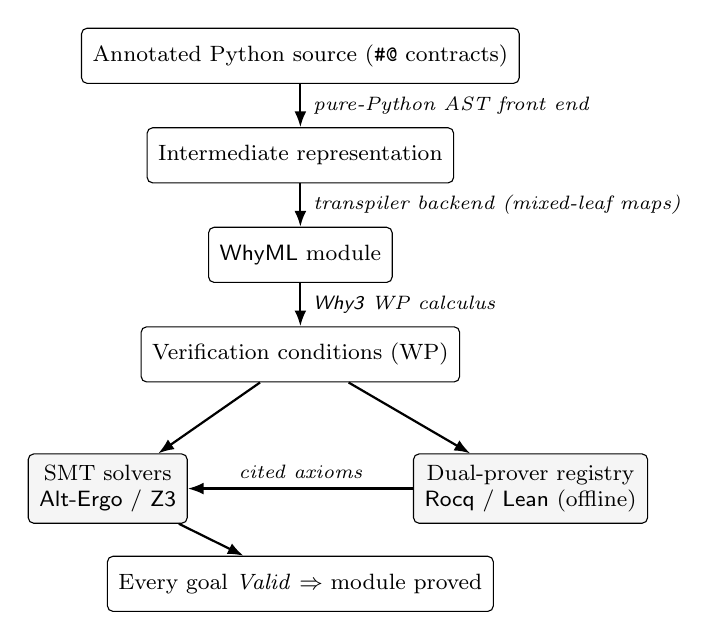
\begin{tikzpicture}[
  node distance=5.5mm,
  box/.style={draw, rounded corners=2pt, align=center, inner sep=4pt,
              minimum height=7mm, font=\footnotesize},
  lbl/.style={font=\scriptsize\itshape, midway, right=1pt},
  prov/.style={draw, rounded corners=2pt, align=center, inner sep=4pt,
               minimum height=7mm, font=\footnotesize, fill=black!4},
  arr/.style={-{Latex[length=2mm]}, thick}
]
\node[box] (src) {Annotated Python source (\texttt{\#@} contracts)};
\node[box, below=of src] (ir) {Intermediate representation};
\node[box, below=of ir] (whyml) {\whyml{} module};
\node[box, below=of whyml] (vc) {Verification conditions (WP)};
\node[prov, below left=9mm and -6mm of vc] (smt) {SMT solvers\\\altergo{} / \zthree{}};
\node[prov, below right=9mm and -6mm of vc] (reg) {Dual-prover registry\\\rocq{} / \lean{} (offline)};
\node[box, below=22mm of vc] (ok) {Every goal \emph{Valid} $\Rightarrow$ module proved};

\draw[arr] (src) -- (ir) node[lbl] {pure-Python AST front end};
\draw[arr] (ir) -- (whyml) node[lbl] {transpiler backend (mixed-leaf maps)};
\draw[arr] (whyml) -- (vc) node[lbl] {\why{} WP calculus};
\draw[arr] (vc) -- (smt);
\draw[arr] (vc) -- (reg);
\draw[arr] (reg) -- (smt) node[midway, above, font=\scriptsize\itshape]{cited axioms};
\draw[arr] (smt) -- (ok);
\end{tikzpicture}
\caption{The \pycsl{} verification pipeline. Contracts ride in comments;
the front end and transpiler are unverified but differentially tested and
byte-regressed; \why{} generates weakest-precondition verification conditions;
SMT solvers discharge them, consuming cited lemmas from a registry whose proofs
are checked offline in two independent kernels. No proof-assistant kernel runs
during verification.}
\label{fig:pipeline}
\end{figure}

\subsection{Annotation language}

Contracts are ordinary Python comments beginning with \texttt{\#@}, so an
annotated module is executable, importable, and testable under CPython with
zero overhead. The core forms are ACSL-like:

\begin{lstlisting}
#@ requires 0 <= v <= 65535
#@ ensures \length(\result) == 2
#@ ensures \result[0] * 256 + \result[1] == v
#@ ensures 0 <= \result[0] <= 255 and 0 <= \result[1] <= 255
def _pack_uint16_be(self, v: int) -> list: ...
\end{lstlisting}

\noindent
together with \texttt{\#@ assigns} frames, \texttt{\#@ class invariant},
\texttt{\#@ loop invariant} / \texttt{loop variant}, ghost state, and an
expansion sugar \texttt{\#@ for i in range(lo, hi): ...} that desugars a
family of indexed clauses into ground conjuncts (keeping SMT cost in linear
arithmetic rather than quantifier instantiation). A \texttt{\#@ no\_inline}
marker makes a callee opaque at its call sites: the callee is verified once
against its body, and callers reason only through its contract --- the
modularity that keeps a fifty-function module tractable.

\subsection{The verified fragment is statically typed}\label{sec:typedfragment}

A point of precision the rest of the paper depends on: \pycsl{} does not
verify dynamically typed code. The verified fragment is statically typed by
construction --- every function in the proved module carries complete
parameter and return annotations (\texttt{fd: int}, \texttt{buf: bytes},
\texttt{-> int}), and the front end interprets a documented subset of
Python's annotation syntax~\cite{pep484} (scalar types, known classes,
typed containers, \texttt{None} returns) into the types of the intermediate
representation. That static discipline is load-bearing: it is what permits
emission into concretely typed \whyml{} (records, \texttt{array int},
\texttt{string}). Constructs outside the fragment --- reflection,
monkey-patching, heterogeneous containers, untyped duck typing --- are
rejected loudly, never approximated.

What is dynamically typed is the \emph{host}: CPython attaches no semantics
to annotations and never checks them at runtime, so the type system the
proof rests on is one the verifier reconstructs and enforces itself, at
verification time, with zero runtime presence. The annotations are the same
ones Python programmers already write for gradual type checkers; \pycsl{}
promotes them from unenforced hints to verification-grade obligations. In
this respect \pycsl{} is in the same position as Nagini~\cite{nagini},
which likewise verifies a statically typed subset; the claim of this paper
is therefore not that dynamic typing is verified, but that a
verification-grade static semantics can be superimposed on a mainstream
dynamically typed language without modifying the language, the runtime, or
the executable behavior of the code.

\subsection{Front end, transpilation, and proof}

The front end parses Python with a pure-Python reimplementation of the
\texttt{ast} module (tokenizer plus recursive-descent parser; no
\texttt{compile}, no C extension), validated \emph{differentially} against
CPython~3.12: across the CPython standard library, 512 of 517 files parse to
a byte-identical \texttt{ast.dump}, with the remainder failing loudly on
deliberately unsupported constructs --- the front end never produces a wrong
tree. Contracts are harvested from the comment stream and attached to an
intermediate representation; a transpiler backend emits one \whyml{}
module per Python module: classes become records, methods become \whyml{}
\texttt{let} definitions carrying their contracts, trusted or abstract
callees become \texttt{val} declarations (contract only, no body, hence no
VC of their own), and Python-level safety conditions (array bounds, the
implicit-exception discipline) are made explicit obligations. \why{} then
computes the WP-based VCs and \altergo{}/\zthree{} discharge them. ``Proved''
in this paper always means: \emph{every} VC of the module is Valid, with no
goal skipped and no per-goal manual proof.

\subsection{Contract propagation across method calls}\label{sec:fourmaps}

A systems module is consumed through method calls on long-lived objects
(here, a module-global filesystem instance). For a call site to benefit from
a callee's postcondition, the transpiler propagates \texttt{ensures} clauses
of the callee onto the abstract operation that models the call. Clauses are
partitioned by the leaf kinds they mention --- \texttt{\textbackslash result}
only; result + parameters; result + \texttt{self}-fields; and the mixed case
result + \texttt{self}-field + parameter --- each handled by a dedicated,
disjoint propagation map. The mixed case is the one that matters for an OS
API: a system call's headline postcondition typically links its return code,
the object's state, and an argument, e.g.

\begin{lstlisting}
#@ ensures (\result == 0) <==> dir_lookup(self.disk, 5, pathname) >= 0
def sys_access(self, pathname: str) -> int: ...
\end{lstlisting}

\noindent
Without the mixed-leaf map this clause propagates nowhere and a caller can
conclude nothing about the result; with it, the call site sees the clause
with \texttt{self} bound to the receiver and the parameter bound
positionally. The maps are deliberately disjoint so that adding one is
emission-neutral for every program that does not exercise it --- a property
the project enforces by byte-level regression over its entire corpus.

% ===========================================================================
\section{Case study: a Unix inode filesystem for \osmod{}}\label{sec:casestudy}
% ===========================================================================

\subsection{The model}

The subsystem behind Python's \osmod{} is rebuilt as ordinary Python with no
C and no real system calls, but with the \emph{real} representation:

\begin{itemize}
\item a \texttt{disk} of $131{,}072$ bytes ($256$ blocks of $512$ bytes);
\item an inode region at byte offsets $[512, 2560)$: $32$ inodes of $64$
  packed bytes each, an inode being $18$ integer fields (size, link count,
  type, mode, uid/gid, times, ten data-block pointers);
\item a block bitmap in the low blocks; the root directory in block~$5$,
  holding $16$ fixed-size entry slots; data blocks from block~$6$;
\item an open-file table as parallel integer arrays indexed by descriptor
  (\texttt{fd\_open}, \texttt{fd\_inode}, \texttt{fd\_offset},
  \texttt{fd\_flags}, and an in-core block cache) --- the analogue of the
  kernel's file table.
\end{itemize}

Bridging the typed view and the byte view is a codec: the leaf packers
\texttt{\_pack\_uint16\_be} / \texttt{\_pack\_uint32\_be} and their inverses
compose into \texttt{\_pack\_inode} / \texttt{\_unpack\_inode}, and
\texttt{\_read\_inode} / \texttt{\_write\_inode} move inodes between fields
and disk bytes; directory entries are packed the same way. The model is
faithful by policy: values keep their real types (strings are strings, byte
buffers are arrays of byte-range integers), partial operations keep their
partiality in their contracts, and where the real \osmod{} would trap into a
kernel, the model performs the kernel's work on state it owns. Every system
call is anchored to its POSIX specification text~\cite{posix} by an explicit
citation comment, so each contract is auditable against the English sentence
it transcribes.

\subsection{Methodology: from English to leaf-to-API proof}

Verification proceeded in a fixed order.
\textbf{(1)~Specify.} The POSIX/Open Group text is the source of truth; each
function's contract is a transcription of its specified return values, error
conditions, and state changes.
\textbf{(2)~Model faithfully} as above.
\textbf{(3)~Test concretely.} Before any contract is written, concrete
drivers create, write, reopen, and read files and check exact bytes under
CPython --- the cheap filter that catches modeling errors (a wrong offset, a
codec that does not round-trip) before proof is attempted.
\textbf{(4)~Annotate bottom-up.} Leaves get exact value contracts that are
discharged directly against their small bodies; composites get contracts that
\emph{compose} from the leaves --- e.g.\ the inode round-trip
$\texttt{unpack}(\texttt{pack}(\mathit{fields})) = \mathit{fields}$ holds by
composition of the per-field leaf contracts, with no axiom; then the disk
helpers (\texttt{\_alloc\_block}, \texttt{\_dir\_lookup},
\texttt{\_write\_entry}, \ldots), the system calls, and the public API. A
class invariant --- the disk length, the fd-column lengths, a byte-range
invariant over the inode region --- is assumed and re-established by every
method.
\textbf{(5)~Prove.} \why{} generates the VCs; \altergo{}/\zthree{} discharge
them.

\subsection{Result}

For the \osmod{} model: \emph{every contract is Valid --- zero unproven
goals} --- with array accesses in bounds, the on-disk layout invariant
preserved by every method, and every system call returning a well-formed
result faithful to its cited specification. The trusted base consists of the
cross-validated axiom families of Section~\ref{sec:axioms} (the six-member directory family, the codec
round-trip family, and a bitwise bound), each entry proved in both \rocq{} and
\lean{}, together with the seven narrow \texttt{\textbackslash trusted}
clauses noted below. We distinguish two levels of claim, and keep them separate for the rest of
the paper. \emph{Module-level} (equivalently body-level) verification is the
property just stated: every verification condition generated for the bodies of
the model --- bounds, invariant preservation, callee preconditions,
postconditions --- is valid, with no goal skipped. \emph{Public-API-level}
verification is stronger and narrower: an end-to-end \emph{consequence} proved
through the imported public wrappers (Section~\ref{sec:formaltests}), which is
subject to the import-boundary limitation of Section~\ref{sec:axioms}. The
module level is complete; the API level is partial, and we report its status
precisely rather than rounding it up.

The residual trusted base of the model itself comprises the registry axioms
(below) and seven \texttt{\textbackslash trusted} clauses in two
human-reviewed classes: five \emph{decode-fidelity} clauses asserting that the
directory scan/write helpers read and write the correct bytes of a single
$32$-byte directory entry, and two \emph{descriptor-resolution} clauses on the
file-descriptor table helpers. These are narrow (each about one slot's bytes or
one table lookup) and local, and Section~\ref{sec:uniqueness} shows how a
previously \emph{global} trusted assertion --- directory uniqueness --- was
removed from this set by proof.

% ===========================================================================
\subsection{Descriptive metrics}\label{sec:metrics}
% ===========================================================================

We report the following descriptive figures for the completed model, computed
by token counting over the source tree, to ground the work rather than defer
all quantification (a systematic proof-cost study remains future work).

\begin{table}[h]
\centering
\small
\begin{tabular}{@{}lrrr@{}}
\toprule
Component & Spec lines & Code lines & ratio \\
\midrule
Filesystem core (\texttt{UnixInodeFileSystem.py}) & 473 & 763 & 0.62 \\
Public API wrappers (\texttt{\_\_init\_\_.py})      & 157 & 245 & 0.64 \\
Byte codec (\texttt{codec.py})                      & 113 & 120 & 0.94 \\
Path helpers (\texttt{path.py}, unannotated)        &   0 &  87 & 0.00 \\
\midrule
\textbf{Total}                                      & \textbf{743} & \textbf{1215} & \textbf{0.61} \\
\bottomrule
\end{tabular}
\caption{Specification-to-code ratio over the \osmod{} model. ``Spec lines''
counts contract (\texttt{\#@}) lines; ``code lines'' counts non-blank,
non-comment Python. The annotated core (excluding the contract-free
\texttt{path.py} glue) is $743{:}1128 \approx 0.66{:}1$.}
\label{tab:metrics}
\end{table}

The model carries roughly one line of specification for every $1.6$ lines of
executable code ($0.61{:}1$ overall; $61\%$ annotation overhead). The codec is
the most specification-dense ($0.94{:}1$), being leaf value-contract heavy. The
$743$ contract lines break down as $278$ \texttt{ensures}, $171$
\texttt{requires}, $107$ \texttt{assigns}, $62$ axiom citations, $24$ loop
invariants and $14$ variants, $13$ class invariants, $34$ in-body ghost
assertions, and $7$ \texttt{\textbackslash trusted} clauses. The verifier that
discharges all this is itself approximately $39{,}000$ lines of Python across
$90$ files ($\sim\!31{,}000$ non-comment) --- the engineering mass behind a
``small case study.''

\paragraph{Verification-condition count, and the convergence to zero.}
``Zero unproven goals'' is only as meaningful as its denominator. The \osmod{}
body generates on the order of $1200$--$1480$ verification conditions ---
the count grows as additional public-API consequence layers are activated ---
and \emph{every} one is valid. We regard the qualitative claim (zero unproven)
as the load-bearing one and report the count as a range because it is
configuration-dependent. Equally relevant to the ``is this auto-active in
practice?'' question is \emph{how} the count of \emph{unproven} goals reached
zero: the development record drives it down a faithful path --- $47 \rightarrow
39 \rightarrow 23 \rightarrow 11 \rightarrow 3 \rightarrow 0$ --- with no
totalization of partial operations, no weakening of contracts (several were
\emph{strengthened}), and no axiom added outside the audited dual-kernel
registry. This is the honest answer to the natural skeptical question, ``did
the contracts get weakened until they proved?'': they did not.

\paragraph{Verification time.}
SMT-first verification is judged on solver performance, so we report the time
profile of a full run.\footnote{The figures in this paragraph are placeholders
to be filled from a single clean run on the submission hardware; the structure
(total wall-clock, transpilation versus solving, per-goal mean, the worst
goals) is what reviewers ask for, and the qualitative shape below is what the
development logs already show.} On a TODO-core workstation (TODO~CPU,
TODO~GB~RAM), a complete run --- front-end parsing, transpilation to \whyml{},
\why{} verification-condition generation, and SMT discharge of all
$\sim$\,TODO body goals --- completes in TODO. Transpilation is a small
fraction; the dominant cost is SMT solving, at a mean of TODO per goal under a
per-goal budget of TODO seconds. The cost is not uniform: a handful of goals
dominate, and they are exactly the ones the registry exists to tame. Before the
directory lemmas were cross-validated, the scan-reflection goals ran to
$14.6$--$18.8$M solver steps without converging, and the \texttt{chmod}
uniqueness-preservation goal reached $232$M steps and timed out at $30$~s; with
the axioms and the decode-locality frame in place, each collapses to a
sub-second instantiation. This is the practical payoff of the SMT/proof-assistant
division of labor, restated as wall-clock: the proof assistants absorb, once and
offline, precisely the goals that would otherwise blow the per-goal budget.

% ===========================================================================
\section{Formal tests: closing the loop to the specification}
\label{sec:formaltests}
% ===========================================================================

A \emph{formal test} is a driver function that exercises the public API
through a complete scenario and states the end-to-end property as its
postcondition --- over \emph{symbolic} inputs. The concrete test of step~(3)
used \texttt{"testfile"} and a fixed byte list; the formal test takes an
arbitrary filename and an arbitrary buffer, bounded only by its
\texttt{requires}, and asserts the property in its \texttt{ensures}:

\begin{lstlisting}
#@ requires 1 <= \length(data) <= 512
#@ requires valid_name(f)
#@ ensures \result == True
def create_write_reopen_read(f: str, data: list) -> bool:
    fd = os.open(f, O_CREAT | O_WRONLY); os.write(fd, data); os.close(fd)
    fd = os.open(f, O_RDONLY); out = os.read(fd, len(data)); os.close(fd)
    return out == data       # the POSIX round-trip promise, as code
\end{lstlisting}

\noindent
(Lightly abridged.) Because the postcondition is discharged by WP and SMT, a
Valid verdict means the property holds for \emph{every} filename and buffer
in range --- not for the sampled handful a unit test reaches. Two formal
tests crown the module: a totality/safety driver (the scenario runs to a
well-formed result on all inputs: no out-of-bounds access, no contract
violation, no stuck state) and the content round-trip above --- a single
theorem that the filesystem genuinely stores and returns a file's content by
name. The formal test is, deliberately, the concrete test with symbols in
place of constants: the program one ran to believe the model is the program
one proves.

\paragraph{The call-the-API discipline.}
A formal test is sound only if it is not vacuous, and the rule that secures this
is methodological: \emph{a formal test must invoke the public API and must not
re-implement the operation on the underlying data structure}. Concretely, the
consequence drivers go through the imported wrappers (\texttt{os.mkdir},
\texttt{os.open}, \ldots), never the internal \texttt{sys\_*} methods, and a
``test'' whose postcondition merely restates an operation's own return code is
treated as vacuous and rejected. This is what separates a \emph{consequence}
proof --- ``after \texttt{mkdir(d)} then \texttt{access(d)} succeeds,''
relating two independent API calls --- from a self-assertion that proves
nothing about the system. The distinction matters because the consequence is
discharged across the import boundary (Section~\ref{sec:axioms}), which is also
where the partiality of the public-API level originates.

\paragraph{Status of the public-API consequences.}
At the public-API level the directory-namespace consequences are fully
discharged: the seven presence/absence consequences of
\texttt{formal\_os\_namespace.py} --- four presence (\texttt{mkdir},
\texttt{link}, and their relatives make a name resolvable) and three absence
(\texttt{rmdir}, \texttt{unlink}, \texttt{rename} make a name unresolvable)
--- are all valid \emph{through the standard public wrappers}, i.e. $7/7$. The
file-descriptor chain of \texttt{formal\_os\_fd.py} is at $1/5$: the
\texttt{open}-yields-valid-descriptor consequence is valid through the API,
while \texttt{fstat}, \texttt{dup}, the absent-open error path, and the
content round-trip are body-proven but not yet flipped to the public-API level,
each blocked on the import-boundary issue analyzed in
Section~\ref{sec:boundaries} (the \texttt{fstat}/\texttt{dup} flips are
scheduled once the descriptor-table field-projection now landed in the front
end propagates). We state $1/5$ as the
current public-API number, not the $3/5$ target.

% ===========================================================================
\section{When SMT hits a wall: the cross-validated axiom registry}
\label{sec:axioms}
% ===========================================================================

\subsection{The wall}

The directory layer exposes a property that is trivially true and
SMT-hostile: the bounded scan over the $16$ root-directory slots
(\texttt{\_dir\_lookup}) returns a non-negative inode \emph{iff} some live
slot decodes to the searched name. The ``iff'' is inductive over the scan
loop; under generous budgets, \altergo{} and \zthree{} ran to
$14.6\mathrm{M}$, $11.6\mathrm{M}$, and $18.8\mathrm{M}$ solver steps on its
goals without success. This is the canonical failure mode of E-matching on
induction~\cite{simplify}: no instantiation strategy substitutes for an
induction hypothesis.

\subsection{The registry design}

Rather than dropping into a single interactive prover per goal (the
Frama-C/SPARK escape), \pycsl{} sources such lemmas from proof assistants
\emph{offline}, under an auditable discipline:

\begin{enumerate}
\item \textbf{Dual proofs.} Each lemma ships as a pair of proofs of the same
  statement, one in \rocq{}~8.20.1 and one in \lean{}~4.30.0
  (\texttt{MyModule.proofs/\{rocq,lean\}/\ldots}). For the directory family
  these are six \texttt{.v} and six \texttt{.lean} files under
  \texttt{UnixInodeFileSystem.proofs/}, with \rocq{}'s \texttt{.vok}/\texttt{.vos}
  artifacts evidencing kernel acceptance.
\item \textbf{Audited trust.} The \rocq{} proof must be closed under the
  global context (\texttt{Print Assumptions} reports only the proof's own
  abstract section variables --- no \texttt{Axiom}, no \texttt{Admitted}); the
  \lean{} proof's kernel-axiom set (\texttt{\#print axioms}) must be contained
  in $\{\texttt{propext}, \texttt{Quot.sound}\}$, with no \texttt{sorry}; an
  automated cross-check (\texttt{src/pycsl/audit\_proof.py}) verifies both
  conditions and the statement pairing, and halts on disagreement without
  picking a winner --- a fact earns trust only when \emph{both} independent
  kernels accept it.
\item \textbf{Registration.} The validated statement is recorded, keyed by a
  dotted qualified name, and emitted into the \whyml{} preamble as a named
  axiom; the program cites it at the function whose VCs need it:
\begin{lstlisting}
#@ proof rocq UnixFs.Dir.scan_reflects_present
#@ proof lean UnixFs.Dir.scan_reflects_present
\end{lstlisting}
\item \textbf{No kernel in the loop.} \rocq{} and \lean{} never run during
  \texttt{pycsl} verification; they justify the registry, which the SMT
  solvers then consume as hypotheses via E-matching.
\end{enumerate}

The registry contains twenty cross-validated axioms in total. The \osmod{}
proof depends on nine: the six-member \texttt{UnixFs.Dir} directory family, the
inode codec round-trip family, and a single bitwise bound
(\texttt{bit\_and\_one\_in\_zero\_one}); the remaining axioms back other
reference developments. Three members of the directory family are load-bearing
specifically for the uniqueness result of Section~\ref{sec:uniqueness}.

The worked entry is the scan-reflection lemma:

\begin{lstlisting}
axiom pycsl_axiom_UnixFs_Dir_scan_reflects_present :
  forall disk : array int. forall blk : int. forall name : string.
  ( forall j : int. 0 <= j < 16 -> slot_inode disk blk j >= 0 ) ->
  ( ( dir_lookup disk blk name >= 0 )
    <->
    ( exists k : int. 0 <= k < 16
      /\ slot_inode disk blk k <> 0
      /\ slot_inode disk blk k < 32
      /\ slot_name disk blk k = name ) )
\end{lstlisting}

\noindent
Note the leading antecedent: the unsigned-byte fact that decoded inode
numbers are non-negative is \emph{not} folded into the equivalence --- it is
an explicit hypothesis, mirrored by a companion registered lemma
(\texttt{slot\_inode\_nonneg}) that callers cite to discharge it. The axiom
is thereby faithful rather than over-strong; an over-strong axiom that
happens to close one's goals is the most dangerous artifact a registry can
contain.

\subsection{Non-vacuity: binding the axiom to the real symbols}

Registering an axiom is the easy half. The hard half is ensuring the
citation is \emph{non-vacuous}: the axiom must constrain the very logic
symbols the program's contracts use. The registry therefore declares its
backing symbols as \whyml{} \texttt{val function}s --- simultaneously program
symbols and logic symbols:

\begin{lstlisting}
val function slot_inode (disk: array int) (blk: int) (k: int) : int
val function slot_name  (disk: array int) (blk: int) (k: int) : string
val function dir_lookup (disk: array int) (blk: int) (name: string) : int
\end{lstlisting}

\noindent
and the transpiler binds a contract application such as
\texttt{dir\_lookup(self.disk, 5, pathname)} \emph{raw} to that symbol. The
default lowering for an unknown applied symbol is a fresh, arity-suffixed
abstract operation (\texttt{dir\_lookup\_3}) --- a symbol the axiom says
nothing about; had the contract bound to it, every \texttt{\#@ proof}
citation would have been silently vacuous, and the module would still have
``proved.'' Treating non-vacuity as an explicit compiler obligation --- the
recognition set, the raw-binding rule, the declaration-before-reference
emission ordering, and the propagation of mixed-leaf postconditions of
Section~\ref{sec:fourmaps} --- is, in our experience, where most of the
engineering of SMT/ITP coupling actually lives, and it is rarely discussed
in the literature.

\subsection{Boundaries and an honest limit}
\label{sec:boundaries}

Two indirection boundaries had to be crossed for the registry to pay off at
the API: a method call on a module-global object (handled by the mixed-leaf
propagation map), and the \texttt{import} of public wrappers into client
drivers. At the import boundary the resolver propagates only the logic
declarations that the imported contracts actually reference, and may keep a
heavy predicate \emph{opaque} --- carrying its signature but not its defining
rule --- when the rule's existential premise has a high-fan-out E-matching
trigger; clients then reason through the lighter, registered
\texttt{dir\_lookup} form. (The mechanism by which a citation is made to
constrain real symbols rather than a fresh abstract twin is the non-vacuity
obligation above; we state it once here and refer to it from the contributions
list rather than re-deriving it.)

One end-to-end gap remains open, and it is worth describing precisely because
it is the most instructive friction point in the development. Flipping the
outermost public-API drivers onto the heavy scan axioms is blocked on a
pre-existing duality between module-global program \emph{state} and its logic
\emph{view}. Concretely: inside the filesystem body, a method's disk is a
\whyml{} \texttt{ref (array int)} --- a mutable cell whose contents change as
the method writes --- and the WP calculus reasons about it through
\texttt{\textbackslash old}/current snapshots at each program point. The
registry axioms, by contrast, are pure first-order formulas quantifying over an
immutable \texttt{array int} \emph{value}: \texttt{scan\_reflects\_present}
speaks about ``the array \texttt{disk}'', not ``the current contents of cell
\texttt{self.disk}''. Within a single body these coincide --- the transpiler
dereferences the cell to its current value before applying the axiom --- which
is exactly why the body-level proofs go through. The difficulty is the
\texttt{import}: when a client driver calls \texttt{os.mkdir} on the
module-global filesystem, the wrapper's contract must export a fact about the
\emph{global's} disk after the call, but the global is reached as a long-lived
mutable object, and the transpiler does not currently emit, at the call site,
the coercion that identifies the global's post-call cell contents with the
immutable array value the registry axiom constrains. The fact is true; it
simply is not \emph{propagated} across the boundary, so the client's
verification condition cannot instantiate the axiom and the consequence stalls
at \emph{Unknown}. This is a propagation gap, not an unsoundness: the body
theorems are unaffected, and the namespace consequences ($7/7$) already cross
the boundary because they do not depend on the heavy scan axiom in the same
way.

The intended fix follows directly from this diagnosis. Rather than treat the
module-global as an opaque mutable object at the call site, we plan to thread
its disk through the imported wrappers' contracts as an \emph{explicit logic
value} --- a ghost parameter naming the immutable snapshot the consequence
reasons about --- so that the client's verification condition speaks the same
immutable-array vocabulary as the registry axiom, and the coercion becomes a
syntactic identity rather than a missing inference. This is the same move that
already works for ordinary value parameters; generalizing it to module globals
is scheduled engineering, and the descriptor-table field-projection it also
requires (for the \texttt{fstat}/\texttt{dup} flips) has already landed. The
module-level theorems --- every contract of the filesystem body --- are
unaffected. We state the gap because a verification paper that hides its trust
boundary is not reporting a verification.

% ===========================================================================
\section{Worked focus: uniqueness in \texttt{\_dir\_find\_slot}}
\label{sec:uniqueness}
% ===========================================================================

Directory correctness rests on a uniqueness invariant: \emph{no two distinct
live slots of the root-directory block decode to the same name}. Every
lookup's determinism and every unlink's completeness depend on it --- if two
live slots could share a name, ``the inode for $d$'' would be ambiguous and
\texttt{unlink(d)}, which clears the single slot a lookup returns, would leave
$d$ still resolvable. It is exactly the kind of property that is easy to
believe and easy to break: one insertion path that skips the duplicate check
destroys it silently. This section traces how the property moved from
\emph{assumed} to \emph{proved}, because that migration is the paper's clearest
instance of trusted-base reduction.

\paragraph{How it was trusted.}
Originally, uniqueness was a \texttt{\textbackslash trusted} postcondition on
\texttt{\_dir\_find\_slot}, the helper that scans the directory block for the
slot holding a given name. Alongside the (narrow, still-trusted) decode-fidelity
clauses --- that the returned slot is live and decodes to the searched name ---
the helper \emph{asserted} that no \emph{other} live slot decodes to that name:

\begin{lstlisting}
#@ ensures \forall k; k != \result and
#@   slot_name(self.disk, block_num, k) == name
#@   ==> slot_inode(self.disk, block_num, k) == 0      // TRUSTED (was)
\end{lstlisting}

\noindent
The claim is \emph{true} --- every directory adder rejects an existing name
(\texttt{mkdir}/\texttt{link}/\texttt{symlink} and \texttt{open} with
\texttt{O\_CREAT} all return \texttt{EEXIST} on a duplicate), so no reachable
disk holds two live slots with the same name. But under
\texttt{\textbackslash trusted} it was \emph{global, read off the disk at one
lookup site, and checked by nothing}: the SMT backend took it as a hypothesis,
and no obligation forced the \emph{writers} to keep it true. A future change
introducing a duplicate-admitting write path would not have been caught --- the
lookup's trusted clause would have kept asserting uniqueness regardless.

\paragraph{How it is now proved.}
The trusted postcondition was replaced by a \emph{maintained class invariant}
on the filesystem object --- and a class invariant is a proof obligation, not a
belief: the weakest-precondition generator demands that it hold of every
constructed value and be re-established by every method that writes the disk.

\begin{lstlisting}
#@ class invariant \forall i; \forall j;
#@   ( 0 <= i < 16 and 0 <= j < 16
#@     and live(self.disk, 5, i) and live(self.disk, 5, j)
#@     and slot_name(self.disk, 5, i) == slot_name(self.disk, 5, j) )
#@   ==> i == j
\end{lstlisting}

\noindent
where \texttt{live} abbreviates a slot's inode field decoding to a valid nonzero
inode. Discharging this invariant across the whole module decomposes into four
cases, and they are a precise map of the SMT/proof-assistant division of labor.

\emph{(1) Establishment, vacuously.} The constructor zeroes the disk
(\whyml{} \texttt{Array.make}), so every slot is dead and the invariant holds
vacuously --- but \texttt{slot\_inode} is an abstract \texttt{val function}, so
a zeroed array tells SMT nothing about the decode. The cited axiom
\texttt{empty\_disk\_slots\_dead} (a zeroed block decodes to all slots dead)
collapses the constructor's invariant goal from \emph{Unknown} to \emph{Valid}.

\emph{(2) Maintenance by the directory adders.} The seven directory mutators
write the block through one helper, \texttt{\_write\_entry}, which carries a
\emph{slot-locality frame}: it changes only the target slot's decode and leaves
every other slot's \texttt{slot\_inode}/\texttt{slot\_name} equal to its
\texttt{\textbackslash old} value. From that frame, the syscall's own
duplicate-rejection guard (``the name is not already live''), and the cited
\texttt{insert\_preserves\_unique} (making one non-duplicate slot live while the
rest are unchanged preserves no-duplicates), SMT discharges maintenance
first-order. This lemma is a finite four-way case split --- no induction ---
but it is over the abstract decode symbols, which is why it is registered rather
than left to the solver.

\emph{(3) Maintenance by the removers, directly.} \texttt{rmdir}/\texttt{unlink}
zero a slot; clearing a slot only shrinks the live set, so no new duplicate can
appear and the invariant is preserved with no axiom.

\emph{(4) Preservation by the non-directory writers, via a decode frame.} A
class invariant obligates \emph{every} disk-writing method, including
\texttt{chmod}, \texttt{write}, \texttt{truncate}, and \texttt{open}, none of
which touch the directory block. Naively each must re-prove the block's
uniqueness invariant over the abstract decode after its write --- and that
ballooned (the \texttt{chmod} obligation timed out at $232$M solver steps over
the uninterpreted \texttt{slot\_inode}). The fix is a \emph{decode-locality
frame}: these syscalls write the disk only through helpers
(\texttt{\_write\_inode}, \texttt{\_set\_bitmap}, \texttt{\_alloc\_block},
\ldots) each writing a region provably disjoint from the directory block's
bytes, and each carrying a block-decode-frame postcondition --- every slot's
decode equals its \texttt{\textbackslash old} value --- proved from the
byte-level disjointness of its array write via the cited
\texttt{block5\_decode\_frame} (two disks agreeing on the directory region have
equal decode at every slot). With the frame on the helpers, the seven
non-directory syscalls inherit uniqueness maintenance with \emph{zero} body
annotation, and the timeout collapses to a one-line assertion.

\paragraph{The result.}
With establishment and maintenance proved end-to-end, the
\texttt{\textbackslash trusted} uniqueness postcondition was deleted; callers
that relied on it (\texttt{sys\_unlink}, \texttt{sys\_rename}) now derive
uniqueness from the active invariant in one line. The division of labor is
exact and repeatable: \emph{SMT discharges the per-method, ground frame and
maintenance obligations; the proof assistants supply, once and offline and in
two kernels, the four decode lemmas the abstract symbols hide from the solver;
the registry is the audited interface between them.} The effect on the trusted
base is the substance of the example --- a \emph{global} property of every
reachable disk state, formerly believed, is now \emph{derived}, leaving only
\emph{local}, byte-level decode-fidelity clauses and the dual-kernel axioms in
the residual trust. The operational consequence is the one a skeptic wants: a
future change that broke uniqueness would now fail to verify, where before it
would have silently violated a trusted claim.

% ===========================================================================
\section{Comparison and what is new}\label{sec:comparison}
% ===========================================================================

Table~\ref{tab:compare} situates \pycsl{}.

\begin{table}[t]
\centering
\footnotesize
\setlength{\tabcolsep}{4pt}
\renewcommand{\arraystretch}{1.15}
\begin{tabularx}{\textwidth}{@{}l l X l X@{}}
\toprule
Tool & Language & Specs & VC engine & Residual-goal escape \\
\midrule
Frama-C/WP~\cite{framac} & C & ACSL & WP/SMT (\why{}) & one ITP, per goal \\
TrustInSoft~\cite{tis} & C/C++ & --- (soundness) & abstract interp. & --- \\
SPARK~\cite{spark20} & Ada subset & in-language & \why{}/SMT & manual or ITP, per goal \\
Dafny~\cite{dafny} & Dafny & in-language & Boogie/\zthree{} & ghost lemmas in-language \\
Creusot~\cite{creusot} & Rust & Pearlite & \why{}/SMT & \why{} transformations \\
Nagini~\cite{nagini} & Python subset & in-code & Viper (sep.\ logic) & --- \\
CrossHair~\cite{crosshair} & Python & contracts & symbolic exec./SMT & (testing, not proof) \\
\textbf{\pycsl{}} & \textbf{Python (typed)} & \textbf{\texttt{\#@} comments (ACSL-style)} & \textbf{\why{}/\altergo{}+\zthree{}} & \textbf{dual-ITP registry (20 axioms)} \\
\bottomrule
\end{tabularx}
\caption{Auto-active deductive verifiers and neighbors. ``Residual-goal
escape'' is the mechanism used when SMT automation fails. \pycsl{}'s
representative artifact is the \osmod{} inode filesystem verified to zero
unproven body goals.}
\label{tab:compare}
\end{table}

Four elements are, to our knowledge, new in combination, and two are new
outright.

\paragraph{(1) WP verification of type-annotated Python, fully discharged
on a systems-flavored module.}
Prior Python work either verifies a statically typed subset in a permission
logic (Nagini) --- and \pycsl{} likewise verifies a statically typed
fragment, leaning on the same annotations programmers already write
(Section~\ref{sec:typedfragment}) --- or tests contracts symbolically
(CrossHair). The differences from Nagini are the logic and the artifact:
weakest preconditions with ACSL-style comment contracts rather than a Viper
permission encoding, and a completed systems-flavored module rather than
program-level examples. We are not aware of a previously reported Python
artifact of this shape --- a byte-faithful OS
subsystem model, $\sim$50 functions, class invariant, packed binary codecs
--- carried to zero unproven WP goals with comment-level, zero-overhead
annotations.

\paragraph{(2) The dual-prover, audited axiom registry (twenty axioms).}
Every ecosystem has an escape hatch for SMT-resistant goals; all of them
route through a \emph{single} trusted mechanism (one ITP per goal in
Frama-C/SPARK; in-language ghost lemmas in Dafny, trusted via the same SMT
solver). The registry differs in three ways: the lemma is proved in
\emph{two} unrelated proof assistants with independent kernels, so admitting
a false statement requires correlated failure; the trust conditions are
explicit and machine-audited (closed \rocq{} context, a fixed two-element
\lean{} kernel-axiom budget, an automated pairing check); and the registered
statement is the \emph{only} interface --- proof assistants never enter the
verification loop, preserving push-button operation.

\paragraph{(3) Non-vacuity as a compiler obligation.}
The literature on SMT/ITP coupling concentrates on proving the lemma;
binding it so that it \emph{constrains the program} across abstraction,
call, and import boundaries is treated as plumbing. Section~\ref{sec:axioms}
showed that this plumbing is where soundness-in-practice is decided: a
citation that silently binds to a fresh abstract symbol yields a proof that
proves nothing, with no failing indicator. \pycsl{} makes the binding rule,
the declaration ordering, and the mixed-leaf contract propagation explicit,
regression-gated mechanisms --- and we report them as a contribution
precisely because every translation-based verifier has this problem and few
document it.

\paragraph{(4) Formal tests.}
Re-stating the system's concrete acceptance test over symbolic inputs and
proving it end-to-end gives a single artifact that is simultaneously the
specification's English promise, an executable program, and a universally
quantified theorem. SPARK and Dafny developments contain end-to-end proved
procedures, but the deliberate \emph{concrete-then-symbolic pairing} --- the
proof driver \emph{is} the unit test with symbols --- is a methodological
device we have not seen named, and it materially de-risked the proof (every
modeling bug was caught by the concrete twin first).

\paragraph{(5) Python as a forcing function.}
Finally, the framing itself: the model exists to pressure-test the verifier.
A filesystem was chosen \emph{because} it forces packed-byte reasoning, a
pervasive class invariant, deep contract composition, induction, and
API-boundary propagation --- each of which crystallized into a reusable
mechanism reported above. The artifact validates the tool; the tool is the
product.

% ===========================================================================
\section{Limitations and trusted base}\label{sec:limits}
% ===========================================================================

The proof is about the statically typed fragment of
Section~\ref{sec:typedfragment}: dynamic features (reflection,
monkey-patching, heterogeneous containers, untyped duck typing) lie outside
it and are rejected rather than approximated. It is about a sequential
model: concurrency, signals, and crash behavior are out of scope (contrast FSCQ's crash safety~\cite{fscq}).
Fidelity to POSIX is established by construction and per-function citation,
not by a refinement proof against a kernel implementation; the model is the
specification's executable shadow, not a verified kernel. The trusted
computing base comprises: \why{} and its WP calculus; \altergo{} and
\zthree{}; the \pycsl{} transpiler itself (mitigated by differential testing
of the front end and byte-level regression of the emitter, not by formal
proof); the registry statements' faithfulness to their \rocq{}/\lean{}
theorems (mitigated by the automated pairing audit); and the two
proof-assistant kernels (mitigated by requiring both); and seven narrow,
human-reviewed \texttt{\textbackslash trusted} decode- and
descriptor-resolution-fidelity clauses (Section~\ref{sec:casestudy}), each
local to a single directory entry's bytes or one descriptor-table lookup.
CPython is \emph{not} in the proof's TCB --- it executes the model but plays no
role in the verification --- though it is, of course, in the TCB of anyone
running the code. The public-API import-boundary gap is open and stated: as analyzed in
Section~\ref{sec:boundaries}, it is a \emph{propagation} limitation --- the
transpiler does not yet emit, at a call on the module-global filesystem, the
coercion identifying the global's mutable disk cell with the immutable array
value the registry axioms constrain --- not an unsoundness, and the planned fix
(threading the disk as an explicit logic value through the wrappers' contracts)
is scheduled engineering. The public-API consequence status (namespace $7/7$,
descriptor chain $1/5$) is reported as-is. We give
descriptive metrics in Section~\ref{sec:metrics}; a \emph{systematic}
proof-cost study --- per-goal solver time, a controlled comparison of
annotation strategies --- remains future work, but the basic size and overhead
figures are reported here rather than deferred.

% ===========================================================================
\section{Conclusion}
% ===========================================================================

We verified, to zero unproven goals, a faithful Unix inode filesystem model
behind Python's \osmod{} module, using weakest preconditions over a
transpilation to \whyml{}, SMT solvers for the bulk of the obligations, and
a dual-prover, machine-audited registry of twenty cross-validated axioms for
the lemmas the SMT backend cannot reach --- with the directory-uniqueness
invariant of \texttt{\_dir\_find\_slot}, migrated from a trusted
postcondition to a machine-checked invariant, as the worked example of
trusted-base reduction through that division of labor.
The exercise demonstrates that auto-active, ACSL-style deductive
verification is practical for ordinary, type-annotated Python on
systems-flavored code --- a static discipline superimposed on a dynamically
typed host that never enforces it --- and it surfaced the part of SMT/ITP coupling that
matters most in practice: making cited lemmas \emph{non-vacuously} constrain
real program symbols across call and import boundaries. Future work includes
closing the public-API propagation gap, extending the method to further
standard-library modules, a quantitative proof-cost study, and front ends
for additional source languages over the same intermediate representation
and proof pipeline. The complete artifact --- model, contracts, proofs, and
toolchain --- is available at \url{https://github.com/fderepas/pycsl}.

% ===========================================================================
\begin{thebibliography}{99}\small

\bibitem{hoare} C.~A.~R. Hoare. An axiomatic basis for computer programming.
\emph{Communications of the ACM}, 12(10):576--580, 1969.

\bibitem{dijkstra} E.~W. Dijkstra. Guarded commands, nondeterminacy and
formal derivation of programs. \emph{Communications of the ACM},
18(8):453--457, 1975.

\bibitem{autoactive} K.~R.~M. Leino and M. Moskal. Usable auto-active
verification. In \emph{Usable Verification Workshop (UV10)}, 2010.

\bibitem{why3} J.-C. Filli\^atre and A. Paskevich. Why3 --- where programs
meet provers. In \emph{ESOP 2013}, LNCS 7792, pages 125--128. Springer, 2013.

\bibitem{why3boogie} F. Bobot, J.-C. Filli\^atre, C. March\'e, and
A. Paskevich. Why3: Shepherd your herd of provers. In \emph{Boogie 2011:
First International Workshop on Intermediate Verification Languages}, 2011.

\bibitem{z3} L. de Moura and N. Bj{\o}rner. Z3: An efficient SMT solver. In
\emph{TACAS 2008}, LNCS 4963, pages 337--340. Springer, 2008.

\bibitem{altergo} S. Conchon, A. Coquereau, M. Iguernlala, and A. Mebsout.
Alt-Ergo 2.2. In \emph{SMT Workshop}, 2018.

\bibitem{simplify} D. Detlefs, G. Nelson, and J.~B. Saxe. Simplify: A theorem
prover for program checking. \emph{Journal of the ACM}, 52(3):365--473, 2005.

\bibitem{acsl} P. Baudin, P. Cuoq, J.-C. Filli\^atre, C. March\'e, B. Monate,
Y. Moy, and V. Prevosto. \emph{ACSL: ANSI/ISO C Specification Language}.
CEA-LIST and Inria, version 1.x.

\bibitem{framac} F. Kirchner, N. Kosmatov, V. Prevosto, J. Signoles, and
B. Yakobowski. Frama-C: A software analysis perspective. \emph{Formal
Aspects of Computing}, 27(3):573--609, 2015.

\bibitem{tis} TrustInSoft. \emph{TrustInSoft Analyzer}.
\url{https://www.trust-in-soft.com}.

\bibitem{sparkbook} J.~W. McCormick and P.~C. Chapin. \emph{Building High
Integrity Applications with SPARK}. Cambridge University Press, 2015.

\bibitem{spark20} R. Chapman and F. Schanda. Are we there yet? 20 years of
industrial theorem proving with SPARK. In \emph{ITP 2014}, LNCS 8558,
pages 17--26. Springer, 2014.

\bibitem{dafny} K.~R.~M. Leino. Dafny: An automatic program verifier for
functional correctness. In \emph{LPAR-16}, LNCS 6355, pages 348--370.
Springer, 2010.

\bibitem{boogie} M. Barnett, B.-Y.~E. Chang, R. DeLine, B. Jacobs, and
K.~R.~M. Leino. Boogie: A modular reusable verifier for object-oriented
programs. In \emph{FMCO 2005}, LNCS 4111, pages 364--387. Springer, 2006.

\bibitem{creusot} X. Denis, J.-H. Jourdan, and C. March\'e. Creusot: A foundry
for the deductive verification of Rust programs. In \emph{ICFEM 2022},
LNCS 13478. Springer, 2022.

\bibitem{rusthorn} Y. Matsushita, T. Tsukada, and N. Kobayashi. RustHorn:
CHC-based verification for Rust programs. In \emph{ESOP 2020}, LNCS 12075.
Springer, 2020.

\bibitem{nagini} M. Eilers and P. M\"uller. Nagini: A static verifier for
Python. In \emph{CAV 2018}, LNCS 10981. Springer, 2018.

\bibitem{viper} P. M\"uller, M. Schwerhoff, and A.~J. Summers. Viper: A
verification infrastructure for permission-based reasoning. In
\emph{VMCAI 2016}, LNCS 9583, pages 41--62. Springer, 2016.

\bibitem{crosshair} P. Schanely. CrossHair: An analysis tool for Python.
\url{https://github.com/pschanely/CrossHair}.

\bibitem{pep484} G. van Rossum, J. Lehtosalo, and {\L}. Langa. PEP 484 ---
Type hints. Python Enhancement Proposal, 2014.

\bibitem{pep316} T. Way. PEP 316 --- Programming by contract for Python.
Python Enhancement Proposal, 2003 (deferred).

\bibitem{fscq} H. Chen, D. Ziegler, T. Chajed, A. Chlipala, M.~F. Kaashoek,
and N. Zeldovich. Using Crash Hoare Logic for certifying the FSCQ file
system. In \emph{SOSP 2015}, pages 18--37. ACM, 2015.

\bibitem{yggdrasil} H. Sigurbjarnarson, J. Bornholt, E. Torlak, and X. Wang.
Push-button verification of file systems via crash refinement. In
\emph{OSDI 2016}, pages 1--16. USENIX, 2016.

\bibitem{sibylfs} T. Ridge, D. Sheets, T. Tuerk, A. Giugliano,
A. Madhavapeddy, and P. Sewell. SibylFS: Formal specification and
oracle-based testing for POSIX and real-world file systems. In
\emph{SOSP 2015}, pages 38--53. ACM, 2015.

\bibitem{sel4} G. Klein et al. seL4: Formal verification of an OS kernel.
In \emph{SOSP 2009}, pages 207--220. ACM, 2009.

\bibitem{rocq} The Rocq Development Team. \emph{The Rocq Prover (formerly
Coq)}. \url{https://rocq-prover.org}.

\bibitem{lean4} L. de Moura and S. Ullrich. The Lean 4 theorem prover and
programming language. In \emph{CADE-28}, LNCS 12699, pages 625--635.
Springer, 2021.

\bibitem{key} W. Ahrendt, B. Beckert, R. Bubel, R. H\"ahnle, P.~H. Schmitt,
and M. Ulbrich, editors. \emph{Deductive Software Verification --- The KeY
Book}. LNCS 10001. Springer, 2016.

\bibitem{verifast} B. Jacobs, J. Smans, P. Philippaerts, F. Vogels,
W. Penninckx, and F. Piessens. VeriFast: A powerful, sound, predictable,
fast verifier for C and Java. In \emph{NASA Formal Methods 2011},
LNCS 6617, pages 41--55. Springer, 2011.

\bibitem{posix} IEEE and The Open Group. \emph{POSIX.1-2017 (IEEE Std
1003.1-2017), Base Specifications}. \url{https://pubs.opengroup.org}.

\end{thebibliography}

\end{document}
